\documentclass{beamer}
\setbeamertemplate{navigation symbols}{}
\usepackage[latin1]{inputenc}
\usepackage{setspace,dsfont}
\usepackage{amsmath,amssymb,pdfpages}
\usepackage[longnamesfirst,nonamebreak]{natbib}
\usepackage[english]{babel}
\usepackage{eurosym,multirow,hyperref,cmll}
\usepackage{listings}
\usepackage{verbatim,booktabs}
\usepackage{verbatimbox}

\newcommand{\Lik}{\mathcal{L}}
\newcommand{\lau}{\lambda_u}
\newcommand{\wi}{\underline{w}}
\newcommand{\m}{\mathcal{M}}
\newcommand{\wa}{\overline{w}}
\newcommand{\lae}{\lambda_e}
\newcommand{\1}{\mathbb{1}}
\newcommand{\F}{\mathcal{F}}
\newcommand{\D}{\mathcal{D}}
\newcommand{\f}{\mathfrak{f}}
\newcommand{\E}{\mathbb{E}}
\newcommand{\V}{\mathbb{V}}
\newcommand{\N}{\mathbb{N}}
\newcommand{\Real}{\mathbb{R}}
\newcommand{\X}{\mathcal{X}}
\newcommand{\A}{\mathcal{A}}
\newcommand{\B}{\mathcal{B}}
\newcommand{\hy}{\hat{y}}

\hypersetup{
    colorlinks,%
    citecolor=blue,%
    filecolor=blue,%
    linkcolor=blue,%
    urlcolor=blue,
}
%\usetheme{Boadilla}
%\usetheme{Marburg}
%\usetheme{Hannover}
%\usetheme{Pittsburgh}
%\usetheme{umbc1}
%\usetheme{Montpellier}
%\usetheme{Singapore}
%\usetheme{}
%\usetheme{}
%\lstset {language=C++}

\DeclareMathOperator{\plim}{plim}
\DeclareMathAlphabet{\mathpzc}{OT1}{pzc}{m}{it}

\beamersetuncovermixins{\opaqueness<1>{25}}{\opaqueness<2->{15}}
\begin{document}
\begin{frame}
\title{ECON 613: Applied Econometrics}
\subtitle{Methods for Cross-sectional Data}
\titlepage
\end{frame}

\section{Binary Response Model}

\begin{frame}
\tableofcontents[currentsection] 
\end{frame}


\begin{frame}\frametitle{Introduction}
Binary response models are models where the variable to be explained $y$ is a random variable taking on the values zero and one which indicate whether or not a certain event has occured. 
\begin{itemize}
\item $y=1$ if a person is employed
\item $y=1$ if a family contributes to a charity during a particular year
\item $y=1$ if a firm has a particular type of pension plan
\item $y=1$ if a worker goes to college
\item Regardless of what $y$ stands for, we refer to $y=1$ as a success and $y=0$ as a failure.
\end{itemize}
An OLS regression of $y$ on dependent variables denoted $x$ ignores the discreteness of the dependent variable and does not constrain predicted probabilities to be between zero and one. 
\end{frame}

\begin{frame}\frametitle{Linear Probability Model (1)}
\begin{equation}
P(y=1) = \beta_0 + \beta_1 x_1+ \ldots + \beta_k x_k. 
\end{equation}

\begin{itemize}
\item If $x_1$ is continuous, $\beta_1$ is the change in the probability of success given one unit increase in $x_1$
\item If $x_1$ is discrete, $\beta_1$ is the difference in the probability of success when $x_1 = 1$ and $x_1 = 0$, holding other $x_j$ fixed. 
\end{itemize}
\end{frame}

\begin{frame}\frametitle{Linear Probability Model (2)}
Given that $y$ is a random variable (Bernouilli), we also have
\begin{eqnarray}
E(y \mid x) &=& \beta_0 + \beta_1 x_1+ \ldots + \beta_k x_k. \\
Var(y \mid x) &=& x\beta (1-x\beta) 
\end{eqnarray}
Implications:
\begin{itemize}
\item OLS regression of $y$ on $x_1, x_2, \ldots, x_k$ produces consistent and unbiaised estimators of the $\beta_j$.
\item Heteroskedacticity, which can be dealt with using standard heteroskedasticity-robust standard errors. 
\item Problem: OLS fitted values may not be between zero and one. 
\end{itemize}
\end{frame}

\begin{frame}\frametitle{Maximum Likelihood Estimation: Logit and Probit Models}
For binary outcome data, the dependent variable $y$ takes one of two values. We let 
\begin{equation}
y = \begin{cases} 1, & \mbox{with probability } p \\ 0, & \mbox{with probability } 1-p \end{cases}
\end{equation}

Parametrize conditional probabilities:
\begin{equation}
p_i = F_{\epsilon}(X\beta)
\end{equation}
And, Marginal Effects
\begin{equation}
\dfrac{\partial Pr(y_i=1 \mid x_i)}{\partial x_{ij}}  = F'_{\epsilon}(X\beta) \beta_j
\end{equation}
\end{frame}

\begin{frame}\frametitle{Probit Model (1)}
The probit model corresponds to the case where $F(x)$ is the cumulative standard normal distribution function 
\begin{equation}
\Phi(x) = \dfrac{1}{\sqrt{2\pi}} \int_{-\infty}^x \exp(\tfrac{1}{2}X^2) dX
\end{equation}
Where $F(X\beta) = \Phi(X\beta)$. 
\end{frame}

\begin{frame}\frametitle{Probit Model (2)}
\begin{itemize}
\item Consider the latent approach
\begin{equation}
y^{\star} = X \beta + \epsilon
\end{equation} where $\epsilon \sim N(0,1)$. 
Think of $y^{\star}$ as the net utility associated with some action. If the action yields positive net utility, it is undertaken otherwise it is not. 
\item We would care only about the sign of $y^{\star}$
\begin{equation}
y = \begin{cases} 1, & \mbox{if } p \\ 0, & \mbox{with probability } 1-p \end{cases}
\end{equation}
\item Probabilities
\begin{eqnarray*}
Pr(y=1) &=& Pr(y^{\star} > 0) = Pr(X \beta + \epsilon \geq 0)\\
        &=& Pr( \epsilon \geq -X \beta) = Pr (\epsilon \leq X\beta) = \Phi(X\beta)
\end{eqnarray*}
\end{itemize}
\end{frame}

\begin{frame}\frametitle{Logit Model}
The logit model specifies the cdf function $F(x)$ is now the logistic function

\begin{equation}
\Lambda(x) = \dfrac{1}{1+ \exp(-x)} = \dfrac{exp(x)}{1+ \exp(x)} 
\end{equation}

The logit model is most easily derived by assuming that 
\begin{equation}
\log\Big(\dfrac{P}{1 - P}\Big) = X \beta
\end{equation}
The logarithm of the odds (ratio of two probabilities) is equal to $X\beta$
\end{frame}

\begin{frame}\frametitle{Maximum Likelihood Estimation}
\begin{itemize}
\item Likelihood can not be defined as a joint density function. 
\item Outcome of a Bernouilli trial
\begin{equation}
f(y_i \mid x_i) = p_i^{y_i} (1-p_i)^{1-y_i}
\end{equation}
\item Given the independence of individuals, the likelihood can be written
\begin{equation}
\Lik(\beta)  = \prod_{i=1}^{n} F(x_i\beta)^{y_i} (1-F(x_i\beta))^{1-y_i}
\end{equation}
\end{itemize}
\end{frame}

\begin{frame}\frametitle{Log Likelihood}

\begin{itemize}
\item The log likelihood
\begin{equation}
\log \Lik(\beta) = \sum_{i=1}^n y_i ln F(x_i \beta) + (1-y_i) ln(1-F(x_i \beta))
\end{equation}
\item First order conditions
\begin{equation}
\sum_{i=1}^{n} \dfrac{y_i - F(x_i\beta)}{F(x_i \beta) (1-F(x_i \beta))} F^{'}(x_i \beta)x_i =0
\end{equation}
\end{itemize}
\end{frame}

\begin{frame}\frametitle{Empirical considerations}
\begin{itemize}
\item Probit and logit yield same outcomes. Only difference is how parameters are scaled.
\item The natural metric to compare models is the fitted log-likelihood provided that the models have the same number of parameters.
\item Although estimated parameters are different, marginal effects are quite similar. 
\end{itemize}
\end{frame}

\begin{frame}\frametitle{Pseudo R2}
\begin{equation}
R^2_{\text{Binary}} =  1-  \dfrac{\Lik(\hat{\beta)}}{N[\bar{y} ln \bar{y} + (1-\bar{y}) ln(1-\bar{y})]}
\end{equation}
\end{frame}

\begin{frame}\frametitle{Predicted Outcomes}
\begin{itemize}
\item The criterion $\sum_i(y_i - \hat{y}_i)^2$ gives the number of wrong predictions. 
\begin{itemize}
\item average rule: let $\hat{y}=1$ when $\hat{p} = F(X\beta)>0.5$
\item Receiver Operating Characteristics (ROC) curve plots the fractions of $y=1$ correctly classified against the fractions of $y=0$ incorrectly specified as the cutoffs $\hat{p} = F(X\beta)>c$ varies. 
\end{itemize}
\end{itemize}
\end{frame}

\begin{frame}\frametitle{Example: Describing the data}
{\tiny
\begin{table}[ht]
\centering
\begin{tabular}{llll}
  \toprule 
 & & No Affair & Affair \\ \hline \hline 
 \multirow{2}{*}{Gender} & female & 0.54 & 0.48 \\ 
     & male & 0.46 & 0.52 \\ \\
  \multirow{9}{*}{Age} & 17.5 & 0.01 & 0.02 \\ 
    & 22 & 0.22 & 0.11 \\ 
    & 27 & 0.26 & 0.24 \\ 
    & 32 & 0.17 & 0.25 \\ 
    & 37 & 0.14 & 0.15 \\ 
    & 42 & 0.08 & 0.12 \\ 
    & 47 & 0.04 & 0.05 \\ 
    & 52 & 0.03 & 0.04 \\ 
    & 57 & 0.04 & 0.02 \\ \\
  \multirow{8}{*}{Years Married} & 0.125 & 0.02 & 0.01 \\ 
      & 0.417 & 0.02 & 0.01 \\ 
    & 0.75 & 0.06 & 0.02 \\ 
    & 1.5 & 0.17 & 0.08 \\ 
    & 4 & 0.17 & 0.18 \\ 
    & 7 & 0.13 & 0.15 \\ 
    & 10 & 0.11 & 0.14 \\ 
    & 15 & 0.31 & 0.41 \\ 
  Share &  & 0.75 & 0.25 \\ 
   \bottomrule 
\end{tabular}
\end{table}} 
\end{frame}

\begin{frame}\frametitle{Example: Affairs}
{\tiny
\begin{table}[ht]
\centering
\begin{tabular}{llll}
  \toprule 
 & & No Affair & Affair \\ \hline \hline 
 \multirow{2}{*}{Children} & no & 0.319 & 0.18 \\ 
     & yes & 0.681 & 0.82 \\ \\
  \multirow{5}{*}{Religiousness} & 1 & 0.062 & 0.133 \\ 
    & 2 & 0.273 & 0.273 \\ 
    & 3 & 0.191 & 0.287 \\ 
    & 4 & 0.348 & 0.22 \\ 
    & 5 & 0.126 & 0.087 \\ \\
  \multirow{7}{*}{Education} & 9 & 0.011 & 0.013 \\ 
    & 12 & 0.069 & 0.087 \\ 
    & 14 & 0.264 & 0.233 \\ 
    & 16 & 0.211 & 0.133 \\ 
    & 17 & 0.137 & 0.18 \\ 
    & 18 & 0.175 & 0.22 \\ 
    & 20 & 0.133 & 0.133 \\ 
   \bottomrule 
\end{tabular}
\end{table}
} 
\end{frame}

%\begin{verbatim}
%> options(digits=2)
%> tapply(Affairs$aff,Affairs$gender,mean)
%female   male 
%  0.23   0.27 
%> tapply(Affairs$aff,Affairs$age,mean)
%17.5   22   27   32   37   42   47   52   57 
%0.50 0.14 0.24 0.33 0.26 0.32 0.30 0.29 0.14 
%> tapply(Affairs$aff,Affairs$yearsmarried,mean)
%0.125 0.417  0.75   1.5     4     7    10    15 
%0.091 0.100 0.097 0.136 0.257 0.280 0.300 0.304 
%> tapply(Affairs$aff,Affairs$children,mean)
%  no  yes 
%0.16 0.29 
%> tapply(Affairs$aff,Affairs$religiousness,mean)
%   1    2    3    4    5 
%0.42 0.25 0.33 0.17 0.19 
%> tapply(Affairs$aff,Affairs$education,mean)
%   9   12   14   16   17   18   20 
%0.29 0.30 0.23 0.17 0.30 0.29 0.25 
%\end{verbatim}

\begin{frame}\frametitle{Probit}
\begin{table}[hb!]
\tiny
\begin{center}
\begin{tabular}{l c c c c }
\toprule
 & Model 1 & Model 2 & Model 3 & Model 4 \\
\midrule
(Intercept)                  & $-0.74^{***}$ & $-0.02$     & $-0.18$     & $-0.02$      \\
                             & $(0.08)$      & $(0.51)$    & $(0.52)$    & $(0.81)$     \\
as.factor(gender)male        & $0.14$        & $0.13$      & $0.14$      & $0.21$       \\
                             & $(0.11)$      & $(0.12)$    & $(0.12)$    & $(0.12)$     \\
as.factor(age)22             &               & $-1.12^{*}$ & $-1.07^{*}$ & $-1.45^{*}$  \\
                             &               & $(0.53)$    & $(0.54)$    & $(0.61)$     \\
as.factor(age)27             &               & $-0.76$     & $-0.82$     & $-1.44^{*}$  \\
                             &               & $(0.53)$    & $(0.53)$    & $(0.62)$     \\
as.factor(age)32             &               & $-0.48$     & $-0.60$     & $-1.36^{*}$  \\
                             &               & $(0.53)$    & $(0.53)$    & $(0.63)$     \\
as.factor(age)37             &               & $-0.70$     & $-0.84$     & $-1.79^{**}$ \\
                             &               & $(0.53)$    & $(0.54)$    & $(0.66)$     \\
as.factor(age)42             &               & $-0.50$     & $-0.65$     & $-1.61^{*}$  \\
                             &               & $(0.54)$    & $(0.55)$    & $(0.67)$     \\
as.factor(age)47             &               & $-0.56$     & $-0.68$     & $-1.72^{*}$  \\
                             &               & $(0.58)$    & $(0.59)$    & $(0.71)$     \\
as.factor(age)52             &               & $-0.62$     & $-0.76$     & $-1.75^{*}$  \\
                             &               & $(0.59)$    & $(0.60)$    & $(0.71)$     \\
as.factor(age)57             &               & $-1.17$     & $-1.31^{*}$ & $-2.36^{**}$ \\
                             &               & $(0.62)$    & $(0.62)$    & $(0.74)$     \\
as.factor(children)yes       &               &             & $0.31^{*}$  & $0.11$       \\
                             &               &             & $(0.15)$    & $(0.17)$     \\
as.factor(yearsmarried)0.417 &               &             &             & $0.01$       \\
                             &               &             &             & $(0.77)$     \\
as.factor(yearsmarried)0.75  &               &             &             & $-0.37$      \\
                             &               &             &             & $(0.67)$     \\
as.factor(yearsmarried)1.5   &               &             &             & $0.22$       \\
                             &               &             &             & $(0.56)$     \\
as.factor(yearsmarried)4     &               &             &             & $0.62$       \\
                             &               &             &             & $(0.57)$     \\
\midrule
Log Likelihood               & -336.91       & -327.84     & -325.74     & -319.69      \\
\bottomrule
%\multicolumn{5}{l}{\scriptsize{$^{***}p<0.001$, $^{**}p<0.01$, $^*p<0.05$}}
\end{tabular}
\end{center}
\end{table}
\end{frame}

\begin{frame}\frametitle{Logit}
\begin{table}[hb!]
\tiny
\begin{center}
\begin{tabular}{l c c c c }
\toprule
 & Model 1 & Model 2 & Model 3 & Model 4 \\
\midrule
(Intercept)                  & $-1.22^{***}$ & $-0.03$     & $-0.31$     & $-0.07$      \\
                             & $(0.13)$      & $(0.82)$    & $(0.84)$    & $(1.48)$     \\
as.factor(gender)male        & $0.24$        & $0.21$      & $0.23$      & $0.34$       \\
                             & $(0.19)$      & $(0.20)$    & $(0.20)$    & $(0.21)$     \\
as.factor(age)22             &               & $-1.88^{*}$ & $-1.78^{*}$ & $-2.44^{*}$  \\
                             &               & $(0.86)$    & $(0.87)$    & $(1.05)$     \\
as.factor(age)27             &               & $-1.24$     & $-1.35$     & $-2.41^{*}$  \\
                             &               & $(0.84)$    & $(0.85)$    & $(1.06)$     \\
as.factor(age)32             &               & $-0.77$     & $-0.99$     & $-2.29^{*}$  \\
                             &               & $(0.84)$    & $(0.86)$    & $(1.08)$     \\
as.factor(age)37             &               & $-1.14$     & $-1.38$     & $-2.99^{**}$ \\
                             &               & $(0.86)$    & $(0.88)$    & $(1.13)$     \\
as.factor(age)42             &               & $-0.82$     & $-1.07$     & $-2.70^{*}$  \\
                             &               & $(0.87)$    & $(0.89)$    & $(1.14)$     \\
as.factor(age)47             &               & $-0.90$     & $-1.11$     & $-2.87^{*}$  \\
                             &               & $(0.94)$    & $(0.95)$    & $(1.21)$     \\
as.factor(age)52             &               & $-1.00$     & $-1.26$     & $-2.95^{*}$  \\
                             &               & $(0.95)$    & $(0.97)$    & $(1.21)$     \\
as.factor(age)57             &               & $-1.97$     & $-2.22^{*}$ & $-3.99^{**}$ \\
                             &               & $(1.03)$    & $(1.05)$    & $(1.29)$     \\
as.factor(children)yes       &               &             & $0.54^{*}$  & $0.16$       \\
                             &               &             & $(0.27)$    & $(0.30)$     \\
as.factor(yearsmarried)0.417 &               &             &             & $0.09$       \\
                             &               &             &             & $(1.49)$     \\
as.factor(yearsmarried)0.75  &               &             &             & $-0.50$      \\
                             &               &             &             & $(1.31)$     \\
as.factor(yearsmarried)1.5   &               &             &             & $0.42$       \\
                             &               &             &             & $(1.10)$     \\
as.factor(yearsmarried)4     &               &             &             & $1.11$       \\
                             &               &             &             & $(1.10)$     \\
\midrule
Log Likelihood               & -336.91       & -327.90     & -325.85     & -320.24      \\
\bottomrule
\end{tabular}
\end{center}
\end{table}
\end{frame}



\begin{frame}\frametitle{Probit VS Logit}

\begin{table}[hb!]
\tiny
\begin{center}
\begin{tabular}{l c c }
\toprule
 & Probit & Logit \\
\midrule
(Intercept)                  & $-0.02$      & $-0.07$      \\
                             & $(0.81)$     & $(1.48)$     \\
as.factor(gender)male        & $0.21$       & $0.34$       \\
                             & $(0.12)$     & $(0.21)$     \\
as.factor(age)22             & $-1.45^{*}$  & $-2.44^{*}$  \\
                             & $(0.61)$     & $(1.05)$     \\
as.factor(age)27             & $-1.44^{*}$  & $-2.41^{*}$  \\
                             & $(0.62)$     & $(1.06)$     \\
as.factor(age)32             & $-1.36^{*}$  & $-2.29^{*}$  \\
                             & $(0.63)$     & $(1.08)$     \\
as.factor(age)37             & $-1.79^{**}$ & $-2.99^{**}$ \\
                             & $(0.66)$     & $(1.13)$     \\
as.factor(age)42             & $-1.61^{*}$  & $-2.70^{*}$  \\
                             & $(0.67)$     & $(1.14)$     \\
as.factor(age)47             & $-1.72^{*}$  & $-2.87^{*}$  \\
                             & $(0.71)$     & $(1.21)$     \\
as.factor(age)52             & $-1.75^{*}$  & $-2.95^{*}$  \\
                             & $(0.71)$     & $(1.21)$     \\
as.factor(age)57             & $-2.36^{**}$ & $-3.99^{**}$ \\
                             & $(0.74)$     & $(1.29)$     \\
as.factor(children)yes       & $0.11$       & $0.16$       \\
                             & $(0.17)$     & $(0.30)$     \\
as.factor(yearsmarried)0.417 & $0.01$       & $0.09$       \\
                             & $(0.77)$     & $(1.49)$     \\
\midrule
AIC                          & 675.38       & 676.48       \\
BIC                          & 754.55       & 755.66       \\
Log Likelihood               & -319.69      & -320.24      \\
\bottomrule
\multicolumn{3}{l}{\scriptsize{$^{***}p<0.001$, $^{**}p<0.01$, $^*p<0.05$}}
\end{tabular}
%\caption{Probit Models}
\label{table:coefficients}
\end{center}
\end{table}

\end{frame}



\begin{frame}\frametitle{Identification considerations}
\begin{itemize}
\item $\beta$ is identified up to a scale. 
\item We observe only whether $X\beta + \epsilon > 0$. 
\item Implication for the interpretation of the coefficients. 
\end{itemize}
\end{frame}

\begin{frame}\frametitle{Model Selection}
\begin{itemize}
\item $AIC = 2k - 2 \log \Lik$ 
\item $BIC = \log(n) k - 2 \log \Lik $
\end{itemize}
\end{frame}


\begin{frame}\frametitle{Determinants of Female Labor Supply}
Cross-section data originating from the health survey SOMIPOPS for Switzerland in 1981.

\begin{itemize}
 \item participation Factor: Did the individual participate in the labor force?
 \item income: Logarithm of nonlabor income.
 \item age: Age in decades (years divided by 10).
\item education: Years of formal education.
\item youngkids: Number of young children (under 7 years of age).
\item oldkids:Number of older children (over 7 years of age).
\item foreign Factor: Is the individual a foreigner (i.e., not Swiss)?
\end{itemize}
\end{frame}

\begin{frame}\frametitle{Describing the data (1)}
\begin{figure}
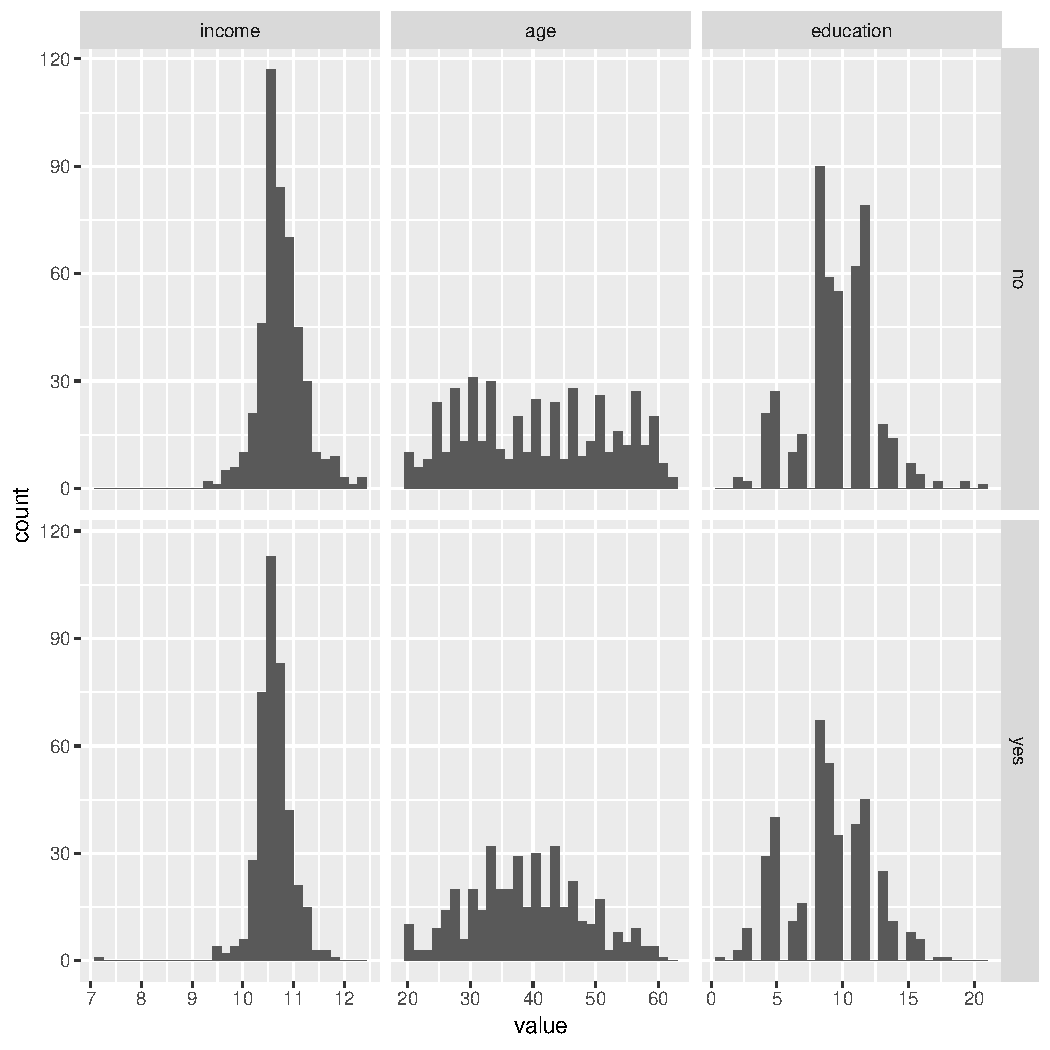
\includegraphics[width = 8cm]{char}
\end{figure}
\end{frame}

\begin{frame}\frametitle{Describing the data (2)}
\begin{table}[ht]
\centering
\begin{tabular}{llll}
  \toprule 
 &  &  \multicolumn{2}{c}{Participation} \\ 
 &  & No  & Yes \\ 
 \multirow{4}{*}{Number of young kids} & 0 & 0.6921 & 0.8454 \\ 
     & 1 & 0.2123 & 0.1172 \\ 
     & 2 & 0.0892 & 0.0324 \\ 
     & 3 & 0.0064 & 0.005 \\ \\
  \multirow{7}{*}{Number of old kids} & 0 & 0.4904 & 0.404 \\ 
     & 1 & 0.2166 & 0.2394 \\ 
     & 2 & 0.2166 & 0.2643 \\ 
     & 3 & 0.0573 & 0.0698 \\ 
     & 4 & 0.0149 & 0.0175 \\ 
     & 5 & 0.0042 & 0 \\ 
     & 6 & 0 & 0.005 \\ 
   \bottomrule 
\end{tabular}
\end{table}
\end{frame}


\begin{frame}\frametitle{Effect of income}

\begin{table}[hb!]
\footnotesize
\begin{center}
\begin{tabular}{l c c c }
\toprule
 & Model 1 & Model 2 & Model 3 \\
\midrule
(Intercept)    & $5.97^{***}$  & $-16.60$    & $116.89$    \\
               & $(1.19)$      & $(10.14)$   & $(67.96)$   \\
income         & $-0.57^{***}$ & $3.69$      & $-37.41$    \\
               & $(0.11)$      & $(1.91)$    & $(20.52)$   \\
$I(income^2)$    &               & $-0.20^{*}$ & $3.97$      \\
               &               & $(0.09)$    & $(2.06)$    \\
$I(income^3)$    &               &             & $-0.14^{*}$ \\
               &               &             & $(0.07)$    \\
\midrule
Log Likelihood & -587.91       & -585.54     & -583.06     \\
Num. obs.      & 872           & 872         & 872         \\
\bottomrule
\multicolumn{4}{l}{\scriptsize{$^{***}p<0.001$, $^{**}p<0.01$, $^*p<0.05$}}
\end{tabular}
%\caption{Probit Models}
\label{table:coefficients}
\end{center}
\end{table}

\end{frame}

\begin{frame}\frametitle{Effect of age}

\begin{table}[hb!]
\footnotesize
\begin{center}
\begin{tabular}{l c c c }
\toprule
 & Model 1 & Model 2 & Model 3 \\
\midrule
(Intercept)    & $0.34^{*}$   & $-3.52^{***}$ & $-1.10$  \\
               & $(0.17)$     & $(0.63)$      & $(2.20)$ \\
age            & $-0.01^{**}$ & $0.19^{***}$  & $-0.00$  \\
               & $(0.00)$     & $(0.03)$      & $(0.18)$ \\
$I(age^2)$       &              & $-0.00^{***}$ & $0.00$   \\
               &              & $(0.00)$      & $(0.00)$ \\
$I(age^3)$       &              &               & $-0.00$  \\
               &              &               & $(0.00)$ \\
\midrule
Log Likelihood & -597.85      & -576.39       & -575.71  \\
Num. obs.      & 872          & 872           & 872      \\
\bottomrule
\multicolumn{4}{l}{\scriptsize{$^{***}p<0.001$, $^{**}p<0.01$, $^*p<0.05$}}
\end{tabular}
%\caption{Probit Models}
\label{table:coefficients}
\end{center}
\end{table}

\end{frame}

\begin{frame}\frametitle{Specification}

\begin{table}[hb!]
\footnotesize
\begin{center}
\begin{tabular}{l c c c }
\toprule
 & Model 1 & Model 2 & Model 3 \\
\midrule
(Intercept)    & $7.66^{***}$  & $4.65^{***}$  & $-7.42$       \\
               & $(1.28)$      & $(1.40)$      & $(10.73)$     \\
income         & $-0.56^{***}$ & $-0.74^{***}$ & $1.55$        \\
               & $(0.12)$      & $(0.13)$      & $(2.03)$      \\
age            & $-0.03^{***}$ & $0.23^{***}$  & $0.23^{***}$  \\
               & $(0.01)$      & $(0.04)$      & $(0.04)$      \\
education      & $-0.03$       & $-0.02$       & $-0.02$       \\
               & $(0.02)$      & $(0.02)$      & $(0.02)$      \\
youngkids      & $-0.71^{***}$ & $-0.64^{***}$ & $-0.64^{***}$ \\
               & $(0.10)$      & $(0.10)$      & $(0.10)$      \\
oldkids        & $-0.01$       & $-0.16^{**}$  & $-0.16^{**}$  \\
               & $(0.04)$      & $(0.05)$      & $(0.05)$      \\
$I(age^2)$       &               & $-0.00^{***}$ & $-0.00^{***}$ \\
               &               & $(0.00)$      & $(0.00)$      \\
$I(income^2)$    &               &               & $-0.11$       \\
               &               &               & $(0.10)$      \\
\midrule
Log Likelihood & -550.08       & -526.38       & -525.86       \\
Num. obs.      & 872           & 872           & 872           \\
\bottomrule
\multicolumn{4}{l}{\scriptsize{$^{***}p<0.001$, $^{**}p<0.01$, $^*p<0.05$}}
\end{tabular}
%\caption{Specification}
\label{table:coefficients}
\end{center}
\end{table}

\end{frame}

\begin{frame}\frametitle{Marginal Effects}
\begin{itemize}
 \item Recall that marginal effects are given by \begin{equation}
\dfrac{\partial Pr(y_i=1 \mid x_i)}{\partial x_{ij}}  = F'_{\epsilon}(X\beta) \beta_j
\end{equation}
\item Different definitions
\begin{itemize}
 \item Average marginal effects in the sample.
 \item Marginal effect evaluated at the mean.
\end{itemize}

\end{itemize}

\end{frame}


\begin{frame}\frametitle{Marginal Effects}
\begin{table}[ht]
\centering
\begin{tabular}{ll}
  \hline
  \hline
  income & 0.53 \\ 
  age & 0.08 \\ 
  education & -0.01 \\ 
  youngkids & -0.22 \\ 
  oldkids & -0.05 \\ 
  I($age^2$) & -0.00 \\ 
  I($income^2$) & -0.04 \\ 
   \hline
\end{tabular}
\end{table}
\end{frame}

\begin{frame}\frametitle{Prediction}
\begin{table}[ht]
\centering
\begin{tabular}{lll}
  \hline
 & \multicolumn{2}{c}{Model}\\ 
Data & 0 & 1 \\ 
  \cline{2-3}
0 & 325 & 146 \\ 
  1 & 137 & 264 \\ 
   \hline
\end{tabular}
\end{table}
\end{frame}

\begin{frame}\frametitle{ROC}
\begin{figure}
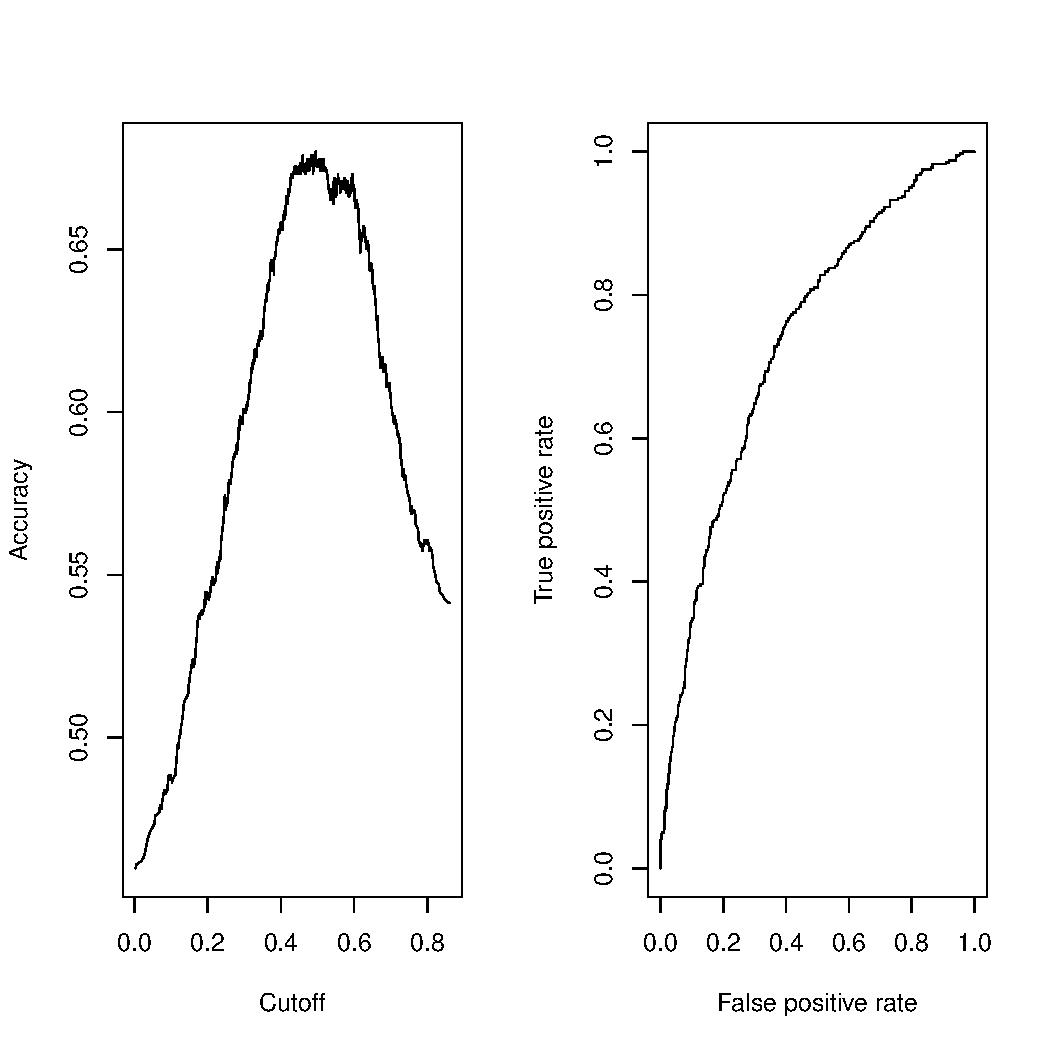
\includegraphics[width = 8cm]{roc}
\end{figure}
\end{frame}

\begin{frame}\frametitle{By citizenship}

\begin{table}[hb!]
\footnotesize
\begin{center}
\begin{tabular}{l c c }
\toprule
 & Native & Immigrants \\
\midrule
(Intercept)    & $-6.85$       & $-67.57$      \\
               & $(11.24)$     & $(48.18)$     \\
income         & $1.17$        & $13.31$       \\
               & $(2.11)$      & $(9.16)$      \\
age            & $0.24^{***}$  & $0.14$        \\
               & $(0.05)$      & $(0.09)$      \\
education      & $0.05^{*}$    & $-0.03$       \\
               & $(0.02)$      & $(0.04)$      \\
youngkids      & $-0.76^{***}$ & $-0.75^{***}$ \\
               & $(0.13)$      & $(0.18)$      \\
oldkids        & $-0.16^{**}$  & $-0.18$       \\
               & $(0.06)$      & $(0.12)$      \\
I($age^2$)       & $-0.00^{***}$ & $-0.00$       \\
               & $(0.00)$      & $(0.00)$      \\
I($income^2$)    & $-0.09$       & $-0.66$       \\
               & $(0.10)$      & $(0.43)$      \\
\midrule
Log Likelihood & -384.24       & -117.82       \\
Num. obs.      & 656           & 216           \\
\bottomrule
\multicolumn{3}{l}{\scriptsize{$^{***}p<0.001$, $^{**}p<0.01$, $^*p<0.05$}}
\end{tabular}
\caption{Probit Models}
\label{table:coefficients}
\end{center}
\end{table}

\end{frame}

\begin{frame}\frametitle{Murder Rates}
Cross-section data on states in 1950.
\begin{itemize}
 \item rate: Murder rate per 100,000 (FBI estimate, 1950).
 \item convictions: Number of convictions divided by number of murders in 1950.
 \item executions: Average number of executions during 1946--1950 divided by convictions in 1950.
\item time: Median time served (in months) of convicted murderers released in 1951.
\item income: Median family income in 1949 (in 1,000 USD).
\item lfp: Labor force participation rate in 1950 (in percent).
\item noncauc: Proportion of population that is non-Caucasian in 1950.
\item southern: Factor indicating region.
\end{itemize}
\end{frame}

\begin{frame}\frametitle{Warnings}
\begin{itemize}
\item Binary model of the determinants of having an execution
\item This is very bad economics
\item An example to illustrate some technical problems
\end{itemize}
\end{frame}

\begin{verbatim}
glm(formula = I(executions > 0) ~ time + income + noncauc + lfp + 
    southern, family = binomial, data = MurderRates)

Coefficients:
              Estimate Std. Error z value Pr(>|z|)  
(Intercept)   10.99326   20.77336   0.529   0.5967  
time           0.01943    0.01040   1.868   0.0617 .
income        10.61013    5.65409   1.877   0.0606 .
noncauc       70.98785   36.41181   1.950   0.0512 .
lfp           -0.66763    0.47668  -1.401   0.1613  
southernyes   17.33126 2872.17069   0.006   0.9952  
---
Signif. codes:  0 �***� 0.001 �**� 0.01 �*� 0.05 �.� 0.1 � � 1
\end{verbatim}

\begin{frame}
\begin{itemize}
 \item Diagnostic
 \item Point estimate and Std.
\end{itemize}

\end{frame}

\begin{verbatim}

table(I(MurderRates$executions > 0), MurderRates$southern)
       
        no yes
  FALSE  9   0
  TRUE  20  15

\end{verbatim}


\begin{frame}\frametitle{Quasi Separation}
\begin{itemize}
 \item We have here $\beta^0$ such that 
\begin{eqnarray*}
 y_i =  0 \quad \text{whenever} \quad x'_i \beta^0 
 \leq 0 \\
  y_i =  1 \quad \text{whenever} \quad x'_i \beta^0 
 \geq 0 \\
\end{eqnarray*}
\item The maximum likelihood estimate does not exist. 
\end{itemize}
\end{frame}

\section{Multinomial Choices}

\begin{frame}
\tableofcontents[currentsection] 
\end{frame}

\begin{frame}\frametitle{Multinomial Models}
Dependent variable has several possible outcomes, that are mutually exclusive
\begin{itemize}
 \item Commute to work (car, bus, bike, walking)
 \item Employment status (full time, part time, unemployed)
 \item Occupation choice, field of study, product choice
\end{itemize}
\begin{itemize}
 \item Ordered choices eg. education choices
 \item Unordered choices eg. fishing mode
\end{itemize}
\end{frame}

\begin{frame}\frametitle{Ordered Discrete Response}
Suppose that $y^{\star}(=x_i\beta + \epsilon_i)$ is continuously distributed with standard deviation $\sigma$ but the observed response $y_i$ is an ordered discrete choice $(ODR)$ taking 0,1,\ldots,R-1 determined by fixed threesholds $\gamma_r$. Formally, we have
\begin{equation}
y = \begin{cases} 0, & \mbox{if } \, x\beta + \epsilon < \gamma_1  \\ 
1, & \mbox{if } \, \gamma_1 \leq x\beta + \epsilon < \gamma_2 \\
2, & \mbox{if } \, \gamma_2 \leq x\beta + \epsilon < \gamma_3 \\
\ldots\\
R-1, & \mbox{if } \, \gamma_{R-1} \leq x\beta + \epsilon 
\end{cases}
\end{equation}
\end{frame}

\begin{frame}\frametitle{Identification}
\begin{itemize}
 \item Not all parameters are identified as in the binary response model.
 \item Consider $\gamma_r \leq x\beta + \epsilon < \gamma_{r+1}$. Then, we have $\dfrac{\gamma_r -\gamma_1}{\sigma} \leq \dfrac{x\beta + \epsilon -\gamma}{\sigma} < \dfrac{\gamma_{r+1} -\gamma_1}{\sigma}$ 
 \item Then, the identified parameters are 
 \begin{eqnarray}
  \alpha = \bigg( \dfrac{\beta_1 - \gamma_1}{\sigma},\dfrac{\beta_2}{\sigma}, \ldots, \dfrac{\beta_k}{\sigma} \bigg)\\
  \rho_r = \dfrac{\gamma_r - \gamma_1}{\sigma}
 \end{eqnarray}
for $r=2,\ldots, R-1$. 
\end{itemize}
\end{frame}

\begin{frame}\frametitle{Toward the Likelihood}
$y=r$
\begin{eqnarray*}
  \gamma_r   &\leq x\beta + \epsilon & < \gamma_{r+1} \\
  \gamma_r - x\beta & \leq \epsilon & < \gamma_{r+1} -x\beta\\
   \dfrac{\gamma_r-\gamma_1}{\sigma} + \dfrac{\gamma_1- x\beta}{\sigma} & \leq \dfrac{\epsilon}{\sigma} & < \dfrac{\gamma_{r+1}-\gamma_1}{\sigma} + \dfrac{\gamma_1-x\beta}{\sigma}\\
     \rho_r - x\alpha  & \leq \dfrac{\epsilon}{\sigma} & < \rho_{r+1} - x\alpha
\end{eqnarray*}
\end{frame}

\begin{frame}\frametitle{Likelihood}
\begin{itemize}
 \item Choice probabilities
\begin{eqnarray*}
   P(y=r \mid x) &=& P(\rho_r - x\alpha\leq \dfrac{\epsilon}{\sigma}  < \rho_{r+1} - x\alpha)\\
        &=& F(\rho_{r+1} - x\alpha) - F(\rho_{r} - x\alpha)
\end{eqnarray*}
\item Likelihood 
\begin{equation}
 \Lik(a,t) = \prod_{i=1}^{N} \prod_{r=0}^{R-1} [P(y_i=r \mid x)]^{y_{ir}}
\end{equation}
\item Log Likelihood of the probit model
\begin{equation}
\log \Lik(a,t) = \sum_{i=1}^{N} \sum_{r=0}^{R-1} y_{ir} \log (\Phi(t_{r+1} - x a) - \Phi(t_{r} - x a))
\end{equation}
where $a$ and $t$ are respectively the parameters to be estimated and the cutoffs. 
\end{itemize}
\end{frame}

\begin{frame}\frametitle{Marginal Effects}
\begin{itemize}
 \item The marginal effects of $x$ on each choice probabilities can be derived as:
\begin{equation}
 \dfrac{\partial P(y=r \mid x)}{\partial x} = -\alpha (\phi(\rho_{r+1} - x\alpha) - \phi(\rho_{r} - x\alpha))
\end{equation}
\item Caution
\begin{equation}
 \sum_{r=0}^{R} P(y=r \mid x)=1 
\end{equation}
Then 
\begin{equation}
 \sum_{r=0}^{R} \dfrac{\partial P(y=r \mid x)}{\partial x} = 0
\end{equation}
An increase in some choice probability necessarily entails a decrease in some other choice probabilities. 
\end{itemize}



\end{frame}

\begin{frame}\frametitle{Multinomial Logit}
The models differ according to whether or not regressors vary across alternatives. 
\begin{itemize}
 \item Conditional logit model
 \begin{equation}
  p_{ij} = \dfrac{\exp(x_{ij}\beta)}{\sum_{l=1}^m \exp(x_{il}\beta)}     \qquad j=1,\ldots,m.
 \end{equation}
 \item Multinomial logit model
  \begin{equation}
  p_{ij} = \dfrac{\exp(x_{i}\beta_j)}{\sum_{l=1}^m \exp(x_{i}\beta_l)}     \qquad j=1,\ldots,m.
 \end{equation}
 \item Mixed logit model
   \begin{equation}
  p_{ij} = \dfrac{\exp(x_{ij}\beta + w_i \gamma_j)}{\sum_{l=1}^m \exp(x_{il}\beta + w_i \gamma_l)}     \qquad j=1,\ldots,m.
 \end{equation}
\end{itemize}
\end{frame}

\begin{frame}\frametitle{Marginal Effects}
\begin{itemize}
 \item Conditional logit
 \begin{equation}
  \dfrac{\partial p_{ij}}{\partial x_{ik}} = p_{ij}(\delta_{ijk}-p_{ik})\beta
 \end{equation}
where $\delta_{ijk}$ is an indicator variable equal to 1 if $j=k$ and equal to 0 otherwise. 
\item Multinomial logit
\begin{equation}
 \dfrac{\partial p_{ij}}{\partial x_{i}} = p_{ij}(\beta_j -\bar{\beta}_i)
\end{equation}
where $\bar{\beta}_i = \sum_{l} p_{il}\beta_l$
\end{itemize}
\end{frame}

\begin{frame}\frametitle{Independence of Irrelevant Alternatives}
\begin{itemize}
 \item A property of the conditional logit and multinomial logit is that discrimination among the m alternatives reduces to a series of pairwise comparisons that are unaffected by the characteristics of alternatives other than the pair under consideration. 
\item The choice probabilities must be unaffected by the removal of one alternative. 
\end{itemize}
That is because
\begin{equation}
 Pr(y=j \mid y=k) = \dfrac{p_j}{p_j + p_k}
\end{equation}
\end{frame}

\begin{frame}\frametitle{Testing for IIA}
\begin{itemize}
 \item Estimate the model twice 
 \begin{itemize}
  \item On the full set of alternatives and obtain $\theta_{full}$ 
  \item On a subset of alternatives and obtain $\theta_{subset}$
 \end{itemize}
\item  Compare $\Lik_{subset}(\theta_{full})$ and $\Lik_{subset}(\theta_{subset})$. If there is a significant different, then IIA is violated.
\end{itemize}
It is very (very) rare that IIA is not violated.
\end{frame}

\begin{frame}\frametitle{Hausman and McFadden Test}

\begin{equation}
 HM = (\hat{\beta}^r - \hat{\beta}^f)^{'}
[var_{\hat{\beta^r}} - var_{\hat{\beta^f}}]^{-1}
 (\hat{\beta}^r - \hat{\beta}^f)
\end{equation}

We have that 

\begin{equation}
 HM \sim \chi^2(|| \beta^r ||)
\end{equation}
 If IIA holds. 
\end{frame}


\begin{frame}\frametitle{Alternatives}
\begin{itemize}
 \item Generalized Extreme Value Model
 \item Nested Logit Model
 \item Random Parameters Logit
 \item Multinomial Probit 
\end{itemize}
\end{frame}

\begin{frame}\frametitle{Nested Logit}
\begin{figure}
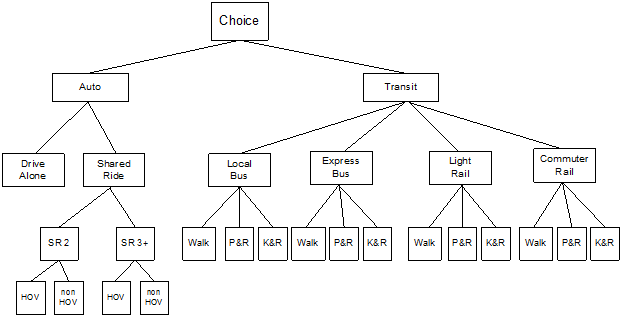
\includegraphics[width = 10cm]{choice}
\end{figure}
\end{frame}

\begin{frame}\frametitle{Nested Logit}
The nested logit model breaks decision making into groups. The utility for the alternative is given
\begin{equation}
 U_{jk} = V_{jk} + \epsilon_{jk} \quad k=1,2,\ldots,K_j, \quad j=1,2,\ldots,J
\end{equation}
Utilities are given by:
\begin{itemize}
 \item $V_{11} + \epsilon_{11}$
 \item $\ldots$
 \item $V_{J K_{J}} + \epsilon_{J K_{J}}$
\end{itemize}

\end{frame}

\begin{frame}\frametitle{Choice Probabilities}
\begin{itemize}
 \item Choice probability
 \begin{equation}
 p_{jk} = p_j \times p_{k \mid j}.
\end{equation}
\item This arises from GEV joint distribution
\begin{equation*}
 F(\epsilon) = exp(-G(e^{-\epsilon_{11}},\ldots,e^{-\epsilon_{1K_{1}}};\ldots;e^{-\epsilon_{J1}},\ldots,e^{-\epsilon_{JK_{J}}}))
\end{equation*}
with 
\begin{equation}
 G(Y) = G(Y_{11},\ldots,Y_{1K_{1}},\ldots,Y_{JK_{J}}) = \sum_{j=1}^{J} \left( \sum_{k=1}^{K_j} Y_{jk}^{\tfrac{1}{\rho_j}}\right)^{\rho_{j}}
\end{equation}
\end{itemize}
\end{frame}

\begin{frame}\frametitle{Model}
Consider
\begin{equation}
 V_{jk} = z_j \alpha + x_{jk}\beta_j \quad k=1,\ldots,K_j, \quad j=1,\ldots,J
\end{equation}

The probability of the nested logit model
\begin{equation*}
p_{jk} = p_j \times p_{k \mid j} = \dfrac{\exp(z_j \alpha + \rho_j I_j)}{\sum_{m=1}^J \exp(z_m\alpha + \rho_m I_m)} \times \dfrac{\exp(x_{jk} \beta / \rho_j + \rho_j I_j)}{\sum_{m=1}^J \exp(z_m\alpha + \rho_m I_m)}
\end{equation*}
where 
\begin{equation*}
 I_j = ln \left( \sum_{l=1}^{K_j} \exp(x_{jl}\beta_j / \rho_j)\right)
\end{equation*}
is the inclusive value or the log-sum.
\end{frame}


\begin{frame}\frametitle{Likelihood}
For the $ith$ observation, we observe $K_1+\ldots+K_J$ outcomes $y_{ijk}$, where $y_{ijk}=1$ if alternative $jk$ is chosen and is zero otherwise. Then the density of one observation $y_i$ can be expressed
\begin{equation*}
 f(y_i) = \prod_{j=1}^{J} \prod_{k=1}^{K_J} [p_{ij} \times p_{ik \mid j}]^{y_{ijk}} = \prod_{j=1}^{J} p_{ij}^{y_{ij}}\left( \prod_{k=1}^{K_J} p_{ik \mid j}^{y_{ijk}} \right)
\end{equation*}
The log likelihood is given by
\begin{equation*}
 ln L = \sum_{i=1}^N \sum_{y=1}^J y_{ij}\log(p_{ij}) +
 \sum_{i=1}^N \sum_{y=1}^J \sum_{k=1}^{K_J} y_{ijk}\log(p_{ik \mid j})
\end{equation*}
\end{frame}

\begin{frame}\frametitle{Discussions and Limitations}
\begin{itemize}
 \item Nested Logit can be estimated in two steps following the construction of the densities
 \item Not all choices are easy to nest.
\end{itemize}
\end{frame}

\begin{frame}\frametitle{Multinomial Probit}
\begin{itemize}
 \item Consider m-choice with
\begin{equation}
 U_j = V_j + \epsilon_j \qquad j=1,2,\ldots,m.
\end{equation}
where $\epsilon \sim \N(0,\Sigma)$. 
\item $\Sigma$ is the matrix of variance-covariance, which can be left unrestricted to capture the correlation between 
choices. 
\item Choice probabilities.. For 4 choices, we have
\begin{equation}
 P(Y=1) = \int_{-\infty}^{-V_{41}} \int_{-\infty}^{-V_{31}}
 \int_{-\infty}^{-V_{21}} f(x,y,z)dzdydx
\end{equation}
where $f(x,y,z)$ is the pdf of the trivariate normal.
\end{itemize}
Need simulation to compute the choice probabilities and the likelihood. 
\end{frame}

\begin{frame}\frametitle{Applications}
\begin{itemize}
 \item Conditional logit
 \item Multinomial logit
 \item Mixed logit
\end{itemize}
\end{frame}

\begin{frame}\frametitle{Data: Car}
Sample of 4654 individuals stating preferences for cars
\begin{itemize}
 \item choice: choice of a vehicule amoung 6 propositions,
 \item college: college education?,
\item hsg2: size of household greater than 2?
\item coml5: commute lower than 5 miles a day?,
\item type: body type, one of regcar (regular car), sportuv (sport utility vehicule), sportcar, stwagon
\item (station wagon), truck, van, for each proposition z from 1 to 6,
\item fuel: fuel for proposition z, one of gasoline, methanol, cng (compressed natural gas), electric.,
\item price: price of vehicule divided by the logarithm of income,
\item range: hundreds of miles vehicule can travel between refuelings/rechargings,
\end{itemize}
\end{frame}

\begin{frame}\frametitle{Data}
\begin{itemize}
\item acc: acceleration, tens of seconds required to reach 30 mph from stop,
\item speed: highest attainable speed in hundreds of mph,
\item pollutionz: tailpipe emissions as fraction of those for new gas vehicule,
\item size: 0 for a mini, 1 for a subcompact, 2 for a compact and 3 for a mid�size or large vehicule,
\item space: fraction of luggage space in comparable new gas vehicule,
\item cost: cost per mile of travel (tens of cents) : home recharging for electric vehicule, station
refueling otherwise,
\item station: fraction of stations that can refuel/recharge vehicule.
\end{itemize}
\end{frame}

\begin{verbatim}
 summary(car[,6:7])
      type             fuel     
 regcar  :10930   gasoline:6958  
 sportuv : 1048   methanol:6952  
 sportcar:  880   cng     :7016  
 stwagon : 4446   electric:6998  
 truck   : 5628                  
 van     : 4992                  
 \end{verbatim}

 \begin{frame}\frametitle{Descriptive Statistics}
\begin{table}[!htbp] \centering 
\tiny
\begin{tabular}{@{\extracolsep{5pt}}lccccccc} 
\\[-1.8ex]\hline 
\hline \\[-1.8ex] 
Statistic  & \multicolumn{1}{c}{Mean} & \multicolumn{1}{c}{St. Dev.} & \multicolumn{1}{c}{Min} & \multicolumn{1}{c}{Pctl(25)} & \multicolumn{1}{c}{Pctl(75)} & \multicolumn{1}{c}{Max} \\ 
\hline \\[-1.8ex] 
college  & 0.429 & 0.514 & 0 & 0 & 1 & 1 \\ 
hsg2  & 0.571 & 0.514 & 0 & 0 & 1 & 1 \\ 
coml5  & 0.429 & 0.514 & 0 & 0 & 1 & 1 \\ 
alt  & 3.214 & 1.805 & 1 & 2 & 4.8 & 6 \\ 
price  & 4.212 & 0.620 & 3.311 & 3.700 & 4.717 & 5.139 \\ 
range  & 275.000 & 79.663 & 125 & 250 & 300 & 400 \\ 
acc  & 4.429 & 1.530 & 2 & 2.9 & 6 & 6 \\ 
speed  & 115.000 & 23.534 & 85 & 95 & 140 & 140 \\ 
pollution  & 0.300 & 0.206 & 0.000 & 0.138 & 0.475 & 0.600 \\ 
size & 2.571 & 0.514 & 2 & 2 & 3 & 3 \\ 
space  & 0.914 & 0.141 & 0.700 & 0.775 & 1.000 & 1.000 \\ 
cost  & 5.714 & 1.729 & 4 & 4 & 7.5 & 8 \\ 
station & 0.371 & 0.421 & 0.000 & 0.100 & 0.825 & 1.000 \\ 
\hline \\[-1.8ex] 
\end{tabular} 
\end{table} 
\end{frame}

\begin{verbnobox}[\small]
Call:
mlogit(formula = choice ~ type + fuel + price + cost + range + acc + speed + pollution + size + space + station, data = car)

nr method
5 iterations, 0h:0m:0s 
successive function values within tolerance limits 

Frequencies of alternatives:
       1        2        3        4        5        6 
0.190589 0.057800 0.288999 0.074989 0.322089 0.065535 

Coefficients :
                 Estimate  Std. Error  z-value  Pr(>|z|)    
2:(intercept) -1.02584508  0.07485823 -13.7038 < 2.2e-16 ***
3:(intercept) -0.58744862  0.09669769  -6.0751 1.239e-09 ***
4:(intercept) -1.81381447  0.11755525 -15.4295 < 2.2e-16 ***
5:(intercept) -1.05078849  0.16094721  -6.5288 6.631e-11 ***
6:(intercept) -2.46225161  0.17963119 -13.7073 < 2.2e-16 ***
typesportuv   -0.00184380  0.15440518  -0.0119 0.9904724    
typesportcar  -0.10424485  0.16602048  -0.6279 0.5300671    
typestwagon   -0.35046787  0.08468066  -4.1387 3.493e-05 ***
typetruck     -0.50135883  0.06291611  -7.9687 1.554e-15 ***
typevan       -0.00736043  0.06849182  -0.1075 0.9144206    
fuelmethanol  -1.01838444  0.23027436  -4.4225 9.757e-06 ***
fuelcng       -0.45483805  0.15971779  -2.8478 0.0044028 ** 
fuelelectric   0.08849715  0.10936308   0.8092 0.4183973    
price         -0.18534361  0.02715810  -6.8246 8.816e-12 ***
cost          -0.07563471  0.00753756 -10.0344 < 2.2e-16 ***
range          0.00349386  0.00026686  13.0927 < 2.2e-16 ***
acc           -0.07628449  0.01108619  -6.8810 5.942e-12 ***
speed          0.00258834  0.00080496   3.2155 0.0013022 ** 
pollution     -0.39984011  0.10192220  -3.9230 8.746e-05 ***
size           0.09364624  0.03020371   3.1005 0.0019320 ** 
space          0.50476619  0.18962883   2.6619 0.0077709 ** 
station        0.37123341  0.09691643   3.8304 0.0001279 ***
\end{verbnobox}

\begin{frame}\frametitle{Interpretation}
\begin{itemize}
 \item Point estimates
 \item Non invariant characteristics
\end{itemize}
\end{frame}


\begin{verbnobox}[\footnotesize]
Call:
mlogit(formula = choice ~ 0 | college + hsg2 + coml5, data = car, 
    method = "nr")

Frequencies of alternatives:
       1        2        3        4        5        6 
0.190589 0.057800 0.288999 0.074989 0.322089 0.065535 

nr method
5 iterations, 0h:0m:2s 
g'(-H)^-1g = 2.73E-05 
successive function values within tolerance limits 

Coefficients :
                Estimate Std. Error z-value  Pr(>|z|)    
2:(intercept) -1.1068260  0.1649744 -6.7091 1.959e-11 ***
3:(intercept)  0.4767147  0.1053347  4.5257 6.019e-06 ***
4:(intercept) -0.9202688  0.1506538 -6.1085 1.006e-09 ***
5:(intercept)  0.6224069  0.1016934  6.1204 9.333e-10 ***
6:(intercept) -0.9056751  0.1510444 -5.9961 2.021e-09 ***
2:college     -0.1277798  0.1661574 -0.7690 0.4418763    
3:college     -0.0021799  0.1061731 -0.0205 0.9836190    
4:college     -0.1369894  0.1504088 -0.9108 0.3624110    
5:college     -0.1606726  0.1021570 -1.5728 0.1157649    
6:college     -0.3907579  0.1510830 -2.5864 0.0096990 ** 
2:hsg2         0.4574850  0.1576870  2.9012 0.0037171 ** 
3:hsg2        -0.0938253  0.1081866 -0.8673 0.3858027    
4:hsg2         0.5734656  0.1420381  4.0374 5.405e-05 ***
5:hsg2        -0.0435102  0.1053016 -0.4132 0.6794633    
6:hsg2         0.5176522  0.1495711  3.4609 0.0005384 ***
2:coml5       -0.3107952  0.1517088 -2.0486 0.0404983 *  
3:coml5       -0.1135059  0.0908377 -1.2495 0.2114658    
4:coml5       -0.1651417  0.1348236 -1.2249 0.2206233    
5:coml5        0.0933282  0.0879897  1.0607 0.2888389    
6:coml5       -0.0084332  0.1389205 -0.0607 0.9515941    
---
Signif. codes:  0 �***� 0.001 �**� 0.01 �*� 0.05 �.� 0.1 � � 1

Log-Likelihood: -7302.8
McFadden R^2:  0.0051045 
Likelihood ratio test : chisq = 74.937 (p.value = 5.8115e-10)
\end{verbnobox}

\begin{frame}\frametitle{Interpretation}
\begin{itemize}
 \item Point estimates
 \item Choice specific characteristics
\end{itemize}
\end{frame}

%\begin{verbnobox}[\footnotesize]
%\end{verbnobox}

\begin{verbnobox}[\footnotesize]
mlogit(formula = choice ~ type + fuel + price + cost + range + 
    acc + speed + pollution + size + space + station | college + 
    hsg2 + coml5, data = car, method = "nr")

Frequencies of alternatives:
       1        2        3        4        5        6 
0.190589 0.057800 0.288999 0.074989 0.322089 0.065535 

nr method
5 iterations, 0h:0m:1s 
g'(-H)^-1g = 0.000103 
successive function values within tolerance limits 

Coefficients :
                 Estimate  Std. Error  z-value  Pr(>|z|)    
2:(intercept) -0.98077920  0.16757969  -5.8526 4.839e-09 ***
3:(intercept) -0.48318237  0.13537617  -3.5692 0.0003581 ***
4:(intercept) -1.87579829  0.18201952 -10.3055 < 2.2e-16 ***
5:(intercept) -0.87144551  0.18284488  -4.7660 1.879e-06 ***
6:(intercept) -2.26014988  0.22614108  -9.9944 < 2.2e-16 ***
typesportuv   -0.02644362  0.15553104  -0.1700 0.8649932    
typesportcar  -0.21869888  0.16998782  -1.2866 0.1982490    
typestwagon   -0.31080773  0.08612210  -3.6089 0.0003075 ***
typetruck     -0.46422781  0.06363490  -7.2952 2.982e-13 ***
typevan        0.07832756  0.06987908   1.1209 0.2623299    
fuelmethanol  -1.10814756  0.23441570  -4.7273 2.276e-06 ***
fuelcng       -0.45210218  0.15988272  -2.8277 0.0046882 ** 
fuelelectric   0.08451873  0.10953658   0.7716 0.4403497    
price         -0.18587114  0.02719289  -6.8353 8.184e-12 ***
cost          -0.07604764  0.00755105 -10.0711 < 2.2e-16 ***
range          0.00350101  0.00026714  13.1055 < 2.2e-16 ***
acc           -0.07754747  0.01111274  -6.9783 2.989e-12 ***
speed          0.00261034  0.00080596   3.2388 0.0012004 ** 
pollution     -0.39126834  0.10210589  -3.8320 0.0001271 ***
size           0.09080954  0.03025242   3.0017 0.0026845 ** 
space          0.51129078  0.18986689   2.6929 0.0070835 ** 
station        0.36589016  0.09697511   3.7730 0.0001613 ***
2:college     -0.10370552  0.16680297  -0.6217 0.5341229    
3:college     -0.06342769  0.10906417  -0.5816 0.5608610    
4:college     -0.15736818  0.15267548  -1.0307 0.3026644    
5:college     -0.21903997  0.10436039  -2.0989 0.0358275 *  
6:college     -0.43115417  0.15332731  -2.8120 0.0049237 ** 
2:hsg2         0.45401801  0.15924012   2.8512 0.0043561 ** 
3:hsg2        -0.09901138  0.11102963  -0.8918 0.3725235    
4:hsg2         0.60397279  0.14515336   4.1609 3.170e-05 ***
5:hsg2        -0.04098946  0.10752259  -0.3812 0.7030421    
6:hsg2         0.53109183  0.15238191   3.4853 0.0004916 ***
2:coml5       -0.32561470  0.15310405  -2.1268 0.0334405 *  
3:coml5       -0.28582517  0.10244637  -2.7900 0.0052708 ** 
4:coml5       -0.23774818  0.14386647  -1.6526 0.0984202 .  
5:coml5       -0.19545405  0.09787761  -1.9969 0.0458336 *  
6:coml5       -0.31954968  0.14602695  -2.1883 0.0286483 *  
---
Signif. codes:  0 �***� 0.001 �**� 0.01 �*� 0.05 �.� 0.1 � � 1

Log-Likelihood: -6968.3
McFadden R^2:  0.050679 
Likelihood ratio test : chisq = 744 (p.value = < 2.22e-16)
\end{verbnobox}



\end{document}


